\section{Theorie}
\label{sec:Theorie}

\subsection{Erzeugung der Röntgenstrahlung}

Eine Strahlung im Energiebereich von etwa 10eV bis 200keV wird als Röntgenstrahlung
bezeichnet. Es können verschiedene Methoden verwendet werden, um diese Strahlung 
zu erzeugen. 
Im vorliegenden Versuchsaufbau erfolgt dies mithilfe beschleunigter
Elektronen, welche an einem Glühdraht durch den glühelektrischen Effekt erzeugt
werden. Die Elektronen werden beschleunigt und auf eine Anode aus einem bestimmten 
Material geschossen, wodurch auf zwei verschiedene Arten Röntgenstrahlung entsteht.

Zunächst ensteht die Bremsstrahlung, bei der die kinetische Energie der Elektronen
durch Ablenkung bzw. Abbremsung in Röntgenstrahlung mit der minimalen Wellenlänge 

\begin{equation}
\lambda_\text{min} = \frac{h c}{e_0 U}
\label{eqn:lambda}
\end{equation}

umgewandelt wird. $h$ beschreibt dabei das Plancksche Wirkungsquantum, $c$ die Lichtgeschwindigkeit
und $U$ die Spannung.
Die kinetische Energie der Elektronen wird dabei nicht immer vollständig in 
Röntgenstrahlung umgewandelt. Deswegen handelt es sich bei der Bremsstrahlung
um ein kontinuierliches Spektrum, welches durch die Wahl der Beschleunigungsspannung
begrenzt wird.

Desweiteren entsteht die durch das Anodenmaterial bestimmte charakteristische 
Strahlung. Diese wird bei der Ionisierung des Atoms durch das Elektron erzeugt. 
Hierbei muss dieses Elektron die äußere Schale eines Atoms auffüllen, so dass bei 
diesem Vorgang Strahlug emittiert wird. 
Aufgrund der diskreten Energieniveaus ergeben sich auch diskrete Frequenzen der
Röntgenstrahlung, die durch 

\begin{equation}
h f = E_\text{m} - E_\text{n}
\end{equation}

gegeben sind. 
Die gängige Notation ist es, die entstehenden Linien im Röntgenspektrum 
beispielsweise mit $K_\alpha$ zu bezeichnen, wobei $K$ die Schale benennt,
in der der Übergang endet, und der Index die Anzahl der gesprungenen Schalen. 
Die Bindungsenergien eines Elektrons auf der n-ten Schale werden dabei im 
Allgemeinen durch die Formel 

\begin{equation}
E_n = -R_{\infty} z_\text{eff}² \frac{1}{n²}
\label{eqn:std}
\end{equation}

beschrieben. 
Hierbei ist $R_\infty$ die Rydbergenergie und $z_\text{eff} = z -\sigma$ die
effektive Kernladung mit der für das jeweilige Elektron im Atom charakteristischen
Abschirmkonstante $\sigma$.
Diese Formel ermöglicht demnach die Bestimmung der Abschirmkonstante $\sigma$
bei bekannten Energien. 

Neben der Hauptquantenzahl $n$ besitzen die Elektronen noch weitere Quantenzahlen,
resultierend aus dem Elektronenspin und dem Bahndrehimpuls, so dass eine weitere,
feinere Aufspaltung der Linien möglich ist. 
Die Energien dieser Feinstruktur lassen sich mithilfe der Sommerfeldschen 
Feinstruktursformel nach 

\begin{equation}
 E_{\text{n}, \text{j}} = -R_{\infty} \left[(z-\sigma_{\text{n}, \text{l}})²\frac{1}{n²}+\alpha²(z-s_{\text{n}, \text{l}})⁴\frac{1}{n³}\left(\frac{1}{j+\frac{1}{2}}-\frac{3}{4n}\right)\right]
\end{equation}

berechnen. Dabei ist $j$ der Gesamtdrehimpuls des Elektrons und $\alpha$ die 
Sommerfeldsche Feinstrukturkonstante. 

\subsection{Absorption von Röntgenstrahlung}

Bei dem Auftreffen von Röntgenstrahlung auf einem Absorber wird diese absorbiert. 
Dabei treten ähnlich wie bei der Erzeugung von Röntgenstrahlung für das Material
charakteristische diskrete Phänomene auf. 
Bei Energien von bis zu ca. $\SI{1}{\mega\electronvolt}$ treten vornehmlich 
Effekte auf, die aus dem Comptoneffekt sowie dem Photoeffekt resultieren. 
Die Fähigkeit zur Absorption, beschrieben durch den Absorptionskoeffizient, 
nimmt mit sinkender Wellenlänge der Röntgenstrahlung ab. 
Bei diskreten Werten treten jedoch Sprünge auf, welche stattfinden, wenn die Energie
der Röntgenstrahlung die Bindungsenergie eines Elektrons der nächsten inneren 
Schale im Absorbermaterial übersteigt. 
In einem solchem Fall treten Absorptionskanten für die Wellenlängen 

\begin{equation}
\lambda_\text{abs} = \frac{h c}{E_\text{n}} - E_\infty
\end{equation}

auf.   
Dabei beschreibt $E-\text{n}-E_infty$ die Bindungsenergie des Elektrons. 
Im vorliegenden Versuch kann die Abschirmkonstante $\sigma_\text{L}$ nach der 
Formel

\begin{equation}
\sigma_L = Z - \left(\frac{4}{\alpha} \sqrt{ \frac{\increment E_\text{L}}{R_\infty}} 
- \frac{5 \increment E_\text{L}}{R_\infty}\right)^{0.5} \left(1 + \frac{19}{32}
\alpha² \frac{\increment E_\text{L}}{R_\infty}\right)^{0.5}
\label{eqn:crap}
\end{equation}

bestimmt werden, wobei $Z$ die Ordnungszahl und $\increment E_\text{L} = E_{\text{L, II}} 
- E_{\text{L, III}}$ die Energiedifferenz zwischen zwei $L$-Kanten ist. 
Die $L_\text{I}$ Kante kann im vorliegenden Versuch wegen zu geringer Auflösung der 
Messtemperatur nicht berücksichtigt werden. 

\subsection{Analyse des Röntgenspektrums über die Bragg-Reflexion}

Um das Röntgenspektrum hinsichtlich seiner Intensität in Abhängigkeit von der 
Wellenlänge untersuchen zu können, wird ein Kristall mit gegebener 
Gitterkonstante $d$ verwendet. 
Die in einem bestimmten Winkel $\theta$ auf den Kristall auftreffende Strahlung
wird, wie in Abbildung \ref{fig:bragg} dargestellt, am Gitter gebeugt, sodass dort ein 
Intensitätsmaximum entsteht. 

\begin{figure}
\centering
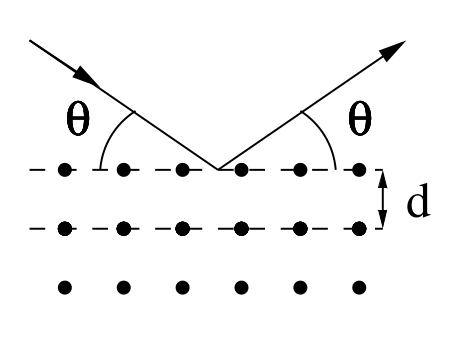
\includegraphics[scale = 0.3]{content/bragg.png}
\caption{Schematische Darstellung der Bragg-Reflexion.[1]}
\label{fig:bragg}
\end{figure}

Für den Glanzwinkel $\theta_\text{glanz}(\lambda)$ tritt konstruktive Interferenz 
auf, sodass die Strahlung hier verstärkt wird. Die Wellenlänge zum zugehörigen 
Winkel lässt sich aus der Bragg-Bedingung zu 

\begin{equation}
\lambda = \frac{2 d \sin{\theta}}{n}
\label{eqn:Bragg}
\end{equation}

bestimmen, wobei $n$ die Ordnung des Maximums beschreibt. 